\documentclass{article}
\usepackage{graphicx}
\usepackage{plantuml}
\usepackage{biblatex}
\usepackage{listings}
\usepackage[most]{tcolorbox} % for creating "note" box
\usepackage{booktabs}

\addbibresource{rpt.bib}

\AtBeginDocument{%
  \DeclareFontShape{TU}{lmr}{m}{scit}{<->ssub*lmr/m/scsl}{}%
}

\newcommand{\loadFig}[2]{{% \inputbetweentag{<tag>}{<filename>}
\begin{figure}[!ht]
    \includegraphics[width=\textwidth,keepaspectratio]{./bckp/fast_tracer/#1.png}
    \caption{#2}
    \label{#1}
\end{figure}}
}% Input file

\newcommand{\loadGraph}[3]{{% \inputbetweentag{<tag>}{<filename>}
\begin{figure}[!ht]
    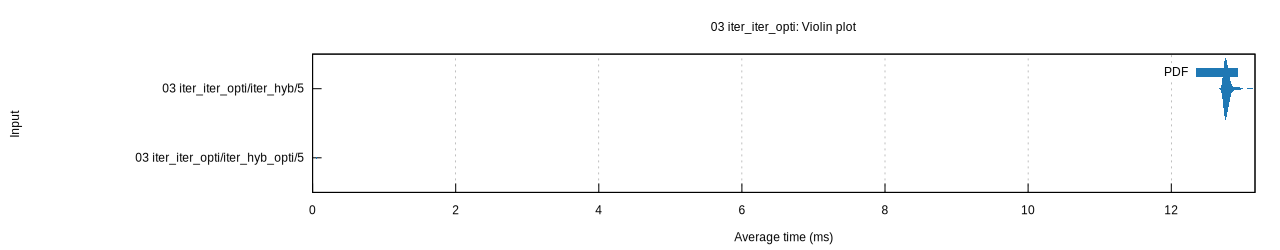
\includegraphics[width=\textwidth,keepaspectratio]{./bckp/criterion/#1/report/violin.png}
    \caption{#3}
    \label{#2}
\end{figure}}
}% Input file

\makeatletter
\NewDocumentCommand{\mynote}{+O{}+m}{%
  \begingroup
  \tcbset{%
    noteshift/.store in=\mynote@shift,
    noteshift=1.5cm
  }
  \begin{tcolorbox}[nobeforeafter,
    enhanced,
    sharp corners,
    toprule=1pt,
    bottomrule=1pt,
    leftrule=0pt,
    rightrule=0pt,
    colback=white!20,
    #1,
    left skip=\mynote@shift,
    right skip=\mynote@shift,
    overlay={\node[right] (mynotenode) at ([xshift=-\mynote@shift]frame.west) {\textbf{Note:}} ;},
    ]
    #2
  \end{tcolorbox}
  \endgroup
  }
\makeatother

\begin{document}

\title{Parallel Systems Project 1}
\author{Karthik Subramanyam CHAKKA}
\date{}

\maketitle

\section{Introduction}
The problem statement is formulated as follows:
Given a $m \times n$ matrix which is sorted in decreasing order both row-wise and column-wise, return the number of negative numbers in grid.

\begin{center}
x = [[4,3,2,-1],[3,2,1,-1],[1,1,-1,-2],[-1,-1,-2,-3]]    
\end{center}
\begin{center}
f(x) = 8
\end{center}

We implement the function $f$ which counts the number of negative numbers in $m \times n$ matrix using methods below:
\begin{itemize}
    \item Iterator-based
    \item Recursion-based
\end{itemize}

In each approach we evaluate performance of algorithms whose nature is:
\begin{itemize}
    \item Sequential
    \item Parallel
    \item Hybrid
    \item Controlled work division(only in recursive approach)
\end{itemize}

Finally we take advantage of the fact that the matrix is sorted and propose an optimization that can be applied to all the aforementioned algorithms.

\section{Implementation}


\subsection{Iterator-based}

This is a brute force approach where each element in the matrix is checked.

\begin{lstlisting}[caption = Iterative]
iter_<type>_1d(row):
    row.<type>_iter().filter(|ele| ele < 0).count()

iter_<type>_2d(matrix):
    matrix.<type>_iter().map(|row| iter_<type>_1d(row)).sum()
\end{lstlisting}
where <type> is sequential, parallel.

\subsubsection{Sequential}
Here normal iterator is used.

\subsubsection{Parallel}
Here parallel iterators from rayon is used.

\loadFig{iter_par_2d}{Iterative Parallel}

Fig \ref{iter_par_2d} shows the execution graph\cite{fast_tracer} obtained using this approach.

\mynote{All the execution graphs presented in this report were obtained by running the code against an input of $64 \times 64$ matrix containing randomly generated numbers in the range $[-100,100]$ arranged in the decreasing order both row-wise and column-wise.
Each distinct color in the graph represents a thread and the block represents work.}

\subsubsection{Hybrid}
Here at the 2d level parallel iterators are used and at the 1d level normal iterators are used.
Hence, threads executing in parallel evaluate their respective rows in sequential manner.

\loadFig{iter_hyb_2d}{Iterative Hybrid}

Fig \ref{iter_hyb_2d} shows the execution graph obtained using this approach.

\subsection{Recursion-based}
\begin{lstlisting}[caption = Recursive]
recur_<type>_1d(row):
    if row.nb_ele == 1:
        return 1 if row[0] < 0 else 0
    else:
        (row_left, row_right) = row.split_at_middle()
        return (recur_<type>_1d(row_left) + 
                recur_<type>_1d(row_right))

recur_<type>_2d(matrix):
    if matrix.nb_rows == 1:
        return recur_<type>_1d(matrix[0])
    else:
        (matrix_top, matrix_bottom) = matrix.split_at_middle()
        return (recur_<type>_2d(matrix_top) + 
                recur_<type>_2d(matrix_bottom))
\end{lstlisting}
where <type> is sequential, parallel.

This is a classic recursive divide and conquer approach coded explicitly.

\subsubsection{Sequential}
Here solving each and every sub-problem and merging of the results is done by just one thread.

\subsubsection{Parallel}
Here rayon's join api is used to achieve parallelism between sub-problems.

\loadFig{recur_par_2d}{Recursive Parallel}

Fig \ref{recur_par_2d} shows the execution graph obtained using this approach.
Here we treat the smallest subproblem as a number. Hence, we can see in the flow graph work is divided into several small units.

\subsubsection{Hybrid}
Here we divide the matrix row-wise between threads executing in parallel and each of the thread executes a single row in a sequential manner.
Hence, we treat a row as the smallest subproblem.

\loadFig{recur_hyb_2d}{Recursive Hybrid}

Fig \ref{recur_hyb_2d} shows the execution graph obtained using this approach.

The row level is executed sequentially in a recursive manner.

\subsubsection{Controlled work division}
\begin{lstlisting}[caption = Controlled work division]
recur_cwd_1d(row, level):
    if lev == 0:
        <approach>_seq_2d(matrix)
    else:
        if row.nb_ele == 1:
            return 1 if row[0] < 0 else 0
        else:
            (row_left, row_right) = row.split_at_middle()
            return( || recur_cwd_1d(row_left, level - 1) + 
                    || recur_cwd_1d(row_right, level - 1))

recur_cwd_2d(matrix, level):
    if lev == 0:
        <approach>_seq_2d(matrix)
    else:
        if matrix.nb_rows == 1:
            return recur_cwd_1d(matrix[0], level - 1)
        else:
            (matrix_top, matrix_bottom) = matrix.split_at_middle()
            return (|| recur_cwd_2d(matrix_top, level - 1) + 
                    || recur_cwd_2d(matrix_bottom, level - 1))
\end{lstlisting}
where <approach> refers to iterative or recursive approach.
Here work is divided into $2^{level}$ units.

\mynote{All the execution graphs of controlled work division apis presented in this report were obtained for level = 3}

\loadFig{recur_cwd_2d}{Controlled work division}

In code an method that solves each subdivision in sequential, iterative manner was chosen.

\subsection{Optimization}
Here we take advantage of the fact that the elements in the matrix are arranged in decreasing order both row and column wise.
\begin{lstlisting}[caption = Optimization]
<approach>_<type>_1d_opti(row):
    if row[0] < 0:
        return row.nb_ele
    else if row[row.nb_ele - 1] >= 0
        return 0
    else:
        << as usual <approach>_<type>_1d(row) >>

<approach>_<type>_2d_opti(matrix):
    if matrix[0][0] < 0:
        return (matrix.nb_cols * matrix.nb_rows)
    else if matrix[matrix.nb_cols -1][matrix.nb_rows -1] >= 0:
        return 0
    else:
        << as usual <approach>_<type>_2d(row) >>
\end{lstlisting}
where <approach> refers to iterative or recursive approach and where <type> is sequential, parallel or hybrid.
With optimization we perform a check at the beginning of the (sub)problem.

For a 2d matrix, if the 1st element is negative, then the whole of the matrix should contain only negative numbers due to the way the matrix is arranged.
Hence, the product of number of columns and rows is returned.
For a row, if the 1st element is negative, then the whole of the row should contain only negative numbers due to the way the matrix is arranged.
Hence, the size of row is returned.
Similarly, if the last element of a matrix or a row is non-negative, then due to the arrangement of matrix it contains only positive numbers.
Hence, zero is returned.

\subsubsection{Iterative}

Fig \ref{iter_par_2d_opti} shows the execution graph obtained using optimization on the iterative approach with parallel iterators at both 2d and 1d level.

\loadFig{iter_par_2d_opti}{Iterative Parallel with Optimization}

Fig \ref{iter_hyb_2d_opti} shows the execution graph obtained using optimization on the iterative approach with parallel iterators only at 2d level.

\loadFig{iter_hyb_2d_opti}{Iterative Hybrid with Optimization}

Here checks are performed only the start/end of the matrix and start/end of the row.

\subsubsection{Recursive}

Fig \ref{recur_par_2d_opti} shows the execution graph obtained using optimization on the recursive approach where the smallest subproblem is a number.

\loadFig{recur_par_2d_opti}{Recursive Parallel with Optimization}

Fig \ref{recur_hyb_2d_opti} shows the execution graph obtained using optimization on the recursive approach where the smallest subproblem is a row.

\loadFig{recur_hyb_2d_opti}{Recursive Hybrid with Optimization}

Fig \ref{recur_cwd_2d_opti} shows the execution graph obtained using optimization on the recursive approach where the smallest subproblem size is controlled by level parameter.

\loadFig{recur_cwd_2d_opti}{Controlled Thread Creation with Optimization}

Here checks are performed at the start/end of every subproblem.
Hence, this would give better gains than optimization as implemented in iterative approach.

\section{Experimentation}
In total 14 apis were implemented, 7 with optimization and 7 without.
Within the 7, 3 were iterator based and 4 were recursion based.

To evaluate the performance a benchmarking framework called Criterion\cite{criterion} is used.
It runs each test for:
\begin{itemize}
    \item 5 seconds if the number of times that the test can be executed within 5 seconds is more than 100 times
    \item 100 times if the time taken to execute the test for 100 times exceeds 5 seconds
\end{itemize}
Hence, every single api is run at least 100 times.
Out of the all the results, 100 samples are picked at random and a 95\% confidence interval plot is generated by the framework.

\subsection{Generation of Ip}
For benchmarking purpose a uniformly distributed matrix is used.
\begin{lstlisting}[caption = Uniform matrix generation]
gen_2d_arr_uni(nb_rows, nb_cols):
    v[nb_rows][nb_cols] = [0]
    for i in nb_rows / 2 -> nb_rows - 1:
        for j in nb_cols / 2 -> nb_cols - 1:
            v[i][j] = -1
    return v
\end{lstlisting}

\subsection{Tests, Observations and Inferences}
8 benchmarks(set of tests) were executed.

\mynote{All the violin plots and tables presented in this report were obtained by running the code against an input of $10000 \times 10000$ matrix containing uniformly distributed values arranged in the decreasing order both row-wise and column-wise.
For controlled work division the level value used is 8}

\subsubsection{Iterator-based}
Runtime of iterator-based code whose execution is sequential, parallel and hybrid is compared as shown in the fig \ref{01_iter} and table \ref{iter}.

\loadGraph{01 iter}{01_iter}{Comparison of Iterator-based methods}
\begin{table}[!ht]
\centering
\begin{tabular}{lc}
\toprule
Label               & Mean Execution Time(ms) \\ \midrule
01 iter/iter\_seq/5 & 27.649                  \\
01 iter/iter\_par/5 & 13.732                  \\
01 iter/iter\_hyb/5 & 12.773                  \\ \bottomrule
\end{tabular}
\caption{Execution time of Iterator-based methods}
\label{iter}
\end{table}

Sequential approach is the slowest as all the work is done by single thread.
Parallel and hybrid approaches are faster due to having multiple threads.
Though there's little overlap in the violin plots of parallel and hybrid approach, in between them hybrid approach seems to be more stable and most of the times faster than parallel.
This happens due to the fact that in parallel approach work related to an individual row(1d) is divided but in hybrid approach work is divided only at matrix(2d) level.
Having too many smaller units of work can be detrimental to performance due to lot of housekeeping code executed.

\subsubsection{Iterator-based with optimization}
Runtime of optimized versions of iterator-based codes are compared as shown in the fig \ref{02_iter_opti} and table \ref{iter_opti}.

\loadGraph{02 iter_opti}{02_iter_opti}{Comparison of Iterator-based methods with optimization}

\mynote{In violin plots if a pdf plot is not visible for a particular test it's due to it's value being significantly smaller than the rest.
In such cases, please check the corresponding table.}

\begin{table}[!ht]
\centering
\begin{tabular}{lc}
\toprule
Label                           & Mean Execution Time(ms) \\ \midrule
02 iter\_opti/iter\_seq\_opti/5 & 14.460                  \\
02 iter\_opti/iter\_par\_opti/5 & 7.689                   \\
02 iter\_opti/iter\_hyb\_opti/5 & 0.058                   \\ \bottomrule
\end{tabular}
\caption{Execution time of Iterator-based methods with optimization}
\label{iter_opti}
\end{table}

The optimization check for sequential and parallel strategies happens at individual row level, whereas for the hybrid strategy it happens at subproblem level.
Hence though the order of execution time between various strategies remains same as without optimization, hybrid approach has significant gain.

\subsubsection{Best of Iterative vs Best of Iterative with optimization}
Runtime of the best of iterative(hybrid) and the best of iterative(hybrid) with optimization is compared as shown in the fig \ref{03_iter_iter_opti} and table \ref{iter_iter_opti}.

\loadGraph{03 iter_iter_opti}{03_iter_iter_opti}{Comparison of Best of Iterative and Best of Iterative with optimization}

\begin{table}[!ht]
\centering
\begin{tabular}{lc}    
\toprule
Label                                & Mean Execution Time(ms) \\ \midrule
03 iter\_iter\_opti/iter\_hyb/5      & 12.772                  \\
03 iter\_iter\_opti/iter\_hyb\_opti/5 & 0.059                   \\ \bottomrule
\end{tabular}
\caption{Execution time of Best of Iterative and Best of Iterative with optimization}
\label{iter_iter_opti}
\end{table}

As expected optimization check skips spending time in whole section of subproblem.
Hence, a method with optimization is faster than without. 

\subsubsection{Recursive}
Runtime of recursion-based code whose execution is sequential, parallel, hybrid and one where work division is controlled are compared as shown in the fig \ref{04_recur} and table \ref{recur}.

\loadGraph{04 recur}{04_recur}{Comparison of Recursion-based methods}

\begin{table}[!ht]
\centering
\begin{tabular}{lc}    
\toprule
Label                 & Mean Execution Time(ms) \\ \midrule
04 recur/recur\_seq/5 & 225.89                  \\
04 recur/recur\_par/5 & 568.11                  \\
04 recur/recur\_hyb/5 & 49.067                  \\
04 recur/recur\_cwd/5 & 12.896                  \\ \bottomrule
\end{tabular}
\caption{Execution time of Recursion-based methods}
\label{recur}
\end{table}

In parallel approach work is forced to be divided to smallest unit possible i,e, a number in the matrix.
Therefore, too much amount of housekeeping code needs to be executed to divide subproblems, and merge results.
Moreover, the deeper the recursion, more work needs to be done by OS to dynamically manage stack growth which also incurs time.
Hence, though parallel strategy can use multiple threads it is slower than sequential one.
The hybrid strategy stops division of work at the row level and executes the row level code sequentially in a recursive manner.
Hence, it enjoys the benefit of parallelism while ensuring that not too much housekeeping code is executed but using recursion to solve row level code will incur costs.
Controlled work division approach restricts the number of subdivisions of work and it solves each subdivision in sequential, iterative manner.
Thus it not only gets the benefit of parallelism but also controls costs of recursion.
Hence, controlled work division approach performs the best.

\subsubsection{Recursive with optimization}
Runtime of optimized versions of recursive-based codes are compared as shown in the fig \ref{05_recur_opti} and table \ref{recur_opti}.

\loadGraph{05 recur_opti}{05_recur_opti}{Comparison of Recursion-based methods with optimization}

\begin{table}[!ht]
\centering
\begin{tabular}{lc}    
\toprule
Label                                & Mean Execution Time(ms) \\ \midrule
05 recur\_opti/recur\_seq\_opti/5 & 0.082                   \\
05 recur\_opti/recur\_par\_opti/5 & 0.111                   \\
05 recur\_opti/recur\_hyb\_opti/5 & 0.080                   \\
05 recur\_opti/recur\_cwd\_opti/5 & 0.039                   \\ \bottomrule
\end{tabular}
\caption{Execution time of Recursion-based methods with optimization}
\label{recur_opti}
\end{table}

In all the approaches the optimization check is performed at the beginning of subproblem.
Hence, there is not any change in the order of execution time of various strategies.

\subsubsection{Best of Recursive vs Best of Recursive with optimization}
Runtime of the best of recursive and the best of recursive with optimization is compared as shown in the fig \ref{06_recur_recur_opti} and table \ref{recur_recur_opti}.

\loadGraph{06 recur_recur_opti}{06_recur_recur_opti}{Comparison of Best of Recursive and Best of Recursive with optimization}

\begin{table}[!ht]
\centering
\begin{tabular}{lc}    
\toprule
Label                                & Mean Execution Time(ms) \\ \midrule
06 recur\_recur\_opti/recur\_cwd/5       & 12.838                 \\
06 recur\_recur\_opti/recur\_cwd\_opti/5 & 0.039                  \\ \bottomrule
\end{tabular}
\caption{Execution time of Best of Recursive and Best of Recursive with optimization}
\label{recur_recur_opti}
\end{table}

Optimization at the level of subproblem eliminates the need to check huge parts of the matrix, hence there's significant gains in speed with optimization.

\subsubsection{Best of Iterator vs Best of Recursive}
Runtime of the best of iterative and the best of recursive is compared as shown in the fig \ref{07_iter_recur} and table \ref{iter_recur}.

\loadGraph{07 iter_recur}{07_iter_recur}{Comparison of Best of Iterator-based and Best of Recursion-based}

\begin{table}[!ht]
\centering
\begin{tabular}{lc}    
\toprule
Label                                & Mean Execution Time(ms) \\ \midrule
07 iter\_recur/iter\_hyb/5  & 12.817                   \\
07 iter\_recur/recur\_cwd/5 & 12.879                   \\ \bottomrule
\end{tabular}
\caption{Execution time of Best of Iterator-based and Best of Recursion-based}
\label{iter_recur}
\end{table}

In iterative hybrid approach rows are not divided and in controlled work division approach division is highly regulated.
Hence, regulation of size of work in both these approaches result in almost similar performance.

\subsubsection{Best of Iterator with optimization vs Best of Recursive with optimization}
Runtime of the best of iterative with optimization and the best of recursive with optimization is compared as shown in the fig \ref{08_iter_recur_opti} and table \ref{iter_recur_opti}.

\loadGraph{08 iter_recur_opti}{08_iter_recur_opti}{Comparison of Best of Iterator-based with optimization and Best of Recursion-based with optimization}

\begin{table}[!ht]
\centering
\begin{tabular}{lc}    
\toprule
Label                                & Mean Execution Time(ms) \\ \midrule
08 iter\_recur\_opti/iter\_hyb\_opti/5  & 0.063                   \\
08 iter\_recur\_opti/recur\_cwd\_opti/5 & 0.041                   \\ \bottomrule
\end{tabular}
\caption{Execution time of Best of Iterator-based with optimization and Best of Recursion-based with optimization}
\label{iter_recur_opti}
\end{table}

Optimization in iterative hybrid approach happens recursively at row level.
Hence subproblem is part of a row and the check can eliminate working on parts of row.
Optimization in controlled work division approach happens recursively at both matrix and row level.
Hence subproblem is part of matrix or a row and the check can eliminate working on not only parts of rows but also whole parts of matrix.
Therefore, recursive controlled work division performs better than iterative hybrid approach.

\section{Conclusion}
From the observations we can see that speed depends on finding a good balance between:
\begin{itemize}
    \item Size of subdivision of work
    \item Depth of recursive calls which can provide control over work division
    \item Dimension(1d row/2d matrix) of subproblem which can take advantage of optimization
\end{itemize}

The optimized recursive approach with controlled work division hits the "sweet" spot between the 3 factors mentioned above.  
Hence, it is the fastest.

\printbibliography

\end{document}